\section{Astrophysics Review}
\subsection{Quantification of Light}
Astrophysical objects are generally studied with \textbf{photometry and spectroscopy.} Studying the light. Since detection gravitational waves are also used but not as commonly.


\textbf{Luminosity} is the total radiative energy output per second. Energy is spread out over a sphere with area $4\pi r^{2}$. Measured in \textbf{ergs}. It is also the \textbf{change in energy over time. }

\begin{equation}
	\label{flux}
	\mbox{Flux}=\frac{L}{4\pi r^{2}}\quad \bigg[\frac{J}{sm^{2}}\bigg] \mbox{\ or } \bigg[\frac{erg}{s cm^{2}}\bigg]
\end{equation}

Flux, or brightness, is also measured as \textbf{magnitude.}

\begin{equation}
	\label{}
	\mbox{\textbf{Apparent Magnitude (m)}}=-2.5\log_{10}\bigg(\frac{F}{F_{0}}\bigg)
\end{equation}
With $F_{0}$ as flux of a star with mag 0. This causes an \textbf{inverse relationship} between magnitude and brightness.


\textbf{Absolute Magnitude (M)}  is the hypothetical magnitude \textbf{if} an object is 10 parsecs away. 



\begin{equation}
	\label{}
	m-M=-2.5\log_{10}\bigg(\frac{F_{obs}}{F_{10pc}}\bigg)
\end{equation}
With $F_{10pc}$ being the flux at 10 parsecs. Using Equation~\ref{flux} this simplifies to
\begin{equation}
	\label{}
	m-M=5\log_{10}\bigg(\frac{d}{10pc}\bigg).
\end{equation}
$m-M$ is the \textbf{distance modulus}, often notated $\mu$


\hfill
\hfill
Usually magnitudes are taken with regard to a certain filter/wavelength. When the magnitude of all wavelengths are considered it is known as the \textbf{bolometric magnitude.}


Generally flux and magnitude are not considered across all emitted wavelengths, and a specific one is chosen. 


\textbf{USEFUL EQUATIONS FROM BoB}
\begin{equation}
	\label{stefan-boltzmann}
	L=4\pi R^{2}\sigma T^{4}
\end{equation}

One parsec is $3.086 \times 10^{16}$m.

\subsection{Stellar Evolution}
\textbf{Herztsprung-Russel Diagram (HR Diagram)} shows the fundamental relationship between stellar temperature, radius, and luminosity.

\hfill

\textbf{Stellar Remnants}

For stars with mass greater than 8 solar masses it becomes a supermassive giant star, undergoes a type II supernova, and becomes a neutron star or black hole

For stars with a mass less than 8 solar masses, becomes an asymptotic giant star, planetary nebula, then white dwarf. 


\section{The Milky Way Galaxy}
Mapping the Milky Way is obviously dominated by finding distances for each body. Magnitudes can be used to find distance:
\begin{equation}
	\label{}
	d=10 \times 10^{\frac{m-M}{5}}
\end{equation}
But different wavelengths of light are absorbed in different proportions from dust, with higher energy light being absorbed more. 

\begin{equation}
	\label{}
	\mbox{observed flux} = f \times  \frac{L}{4\pi d^{2}}
\end{equation}
Where $f$ is the fraction of light transmitted ($f<1$)
\begin{equation}
	\label{}
	F_{obs}=f \cdot F_{10pc}\cdot  \frac{10pc^{2}}{d^{2}}
\end{equation}

\begin{equation}
	\label{}
	m=-2.5\log{f}+M-5\log{10pc}+5\log{d}
\end{equation}
Where $-2.5\log(f)$ is known as the \textbf{extinction in magnitude}. Referred to as $A$. Resolves to

\begin{equation}
	\label{}
	d=10^{\frac{m-M+5}{5}} \cdot 10^{\frac{-A}{5}}
\end{equation}

\subsection{Tully-Fischer and R25 Equations}
\begin{equation}
	\label{}
	M_{B}=-C\log_{10}(V_{max})+B
\end{equation}
C and B Values
\begin{enumerate}
	\item Sa: 9.95, B=3.15
\item Sb: 10.2, B=2.71
\item Sc: 11, B=3.31
\end{enumerate}

\begin{equation}
	\label{}
	\log_{10}(R_{25})=-0.249M_{B}-4
\end{equation}


\subsection{Structure of Milky Way}
Diameter of galactic disk is 50 kpc. Open clusters lie in the plane of the disk, and globular clusters that formed at the same time of the Milky Way inhabit the \textbf{stellar halo}, which is a sphere around the disk.


\subsection{Center of Milky Way Sagittarius A*}
Super massive black hole. First some things about orbits
\begin{equation}
	\label{}
	P^{2}=\frac{4\pi^{2}}{G(M)}r^{3}
\end{equation}
For ellipse use semimajor axis. This is \textbf{Kepler's third law} and is often used to find masses of orbiting bodies. Using this and S\-02, a star that orbits the supermassive black hole, the mass can be calculated to $~3\-4$ million solar masses.

\textbf{Sagittarius A*} emits $~10^{7}L\odot$ of radio emission from infalling material releasing gravitational energy.


\subsection{Distribution of Dark Matter}
Tangential velocities on the outskirts of galaxies are higher than can be accounted for with visible mass in the galaxies. There must be some sort of \textbf{invisible matter}. The distribution of dark matter is modeled by:

\begin{equation}
	\label{}
	\rho(r)=\frac{\rho_{0}}{1+(\frac{r}{a}^{2})}
\end{equation}
With $\rho_{0}$ as a central density and $a$ as a constant that describes change in density per radial increase.

This is then fit to an observed velocity curve. Only applies to large radii, as in farther than most of the visible material. 

A newer formulation of this is 
\begin{equation}
	\label{}
	\rho_{new}(r)=\frac{\rho_{0}}{(\frac{r}{a}(1+\frac{r}{a}^{2}))}
\end{equation}
This works better closer to the galactic center.


\section{Other Galaxies} The most common are \textbf{spiral} and \textbf{elliptical}. Galaxies are typically sorted based on how spiralic and how elliptical it is. B indicates bar in center. 


%\begin{figure}
%	\label{hubblegalaxy}
	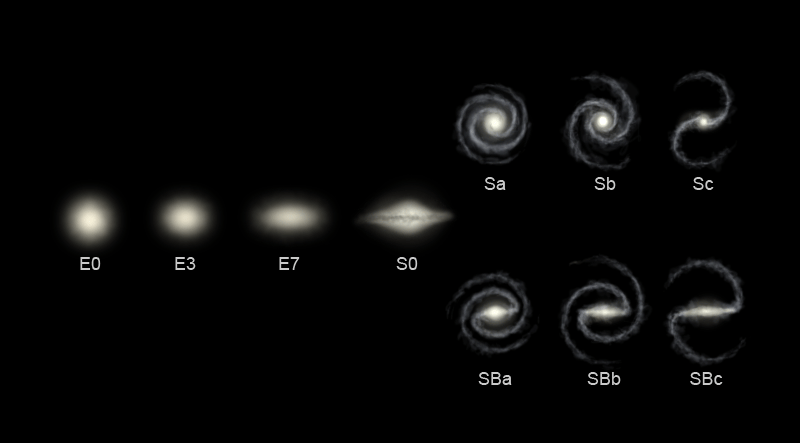
\includegraphics[width=4.5in]{hubblegalaxy.png}
%\end{figure}

Elliptical galaxies are spherical, not discs. Details like eccentricity can be difficult to determine based on their angle to us. As the galaxy as a whole rotates, it becomes more planar. 

Elliptical galaxies are formed likely by merging galaxies. Galaxies with larger bulges (Sa or SBa) have faster velocities on average and \textbf{larger} mass to light ratios than galaxies with smaller bulges (Sc or SBc), meaning a greater nonoptical matter content.








\subsection{Rotation Rate}
A galaxy must not be perpendicular to our line of sight. We measure frequency across a band of the galaxy. One side will be more red and the other bluer. This determines the tangential velocities on the outside of the disk. One can plot flux per radial velocity based on this Doppler shifting, which gives radial velocity relative to us for CoM of the galaxy and how each side is moving relative to the center.

\begin{equation}
	\label{}
	V_{\max}=\frac{v_{obs}}{2\sin{i}}
\end{equation}
With i as the angle of inclination, 0 being perpendicular and 90 being edge on. $V_{obs}$ is the difference in velocity given by difference in doppler shifting and $V_{\max}$ is the maximum tangential velocity of the galaxy, where it evens out. Graph in notebook.


\subsection{Galaxy Interactions}
Galaxies fall into each other's gravitational potentials. This is fundamental for their development, and causes increases in stellar formation. 

\textbf{Dynamical Friction} While there aren't many stellar collisions, a massive body moving through a `field' of other massive bodies causes a gravitational drag. This results in a higher density behind the moving massive body, and the gravity of the bodies in a field behind the moving body cause a net drag known as \textbf{dynamical friction.} Modeling this requires use of an \textbf{N-Body model}: a computational model of $N$ number of masses, modeling the motion of each mass due to gravity.

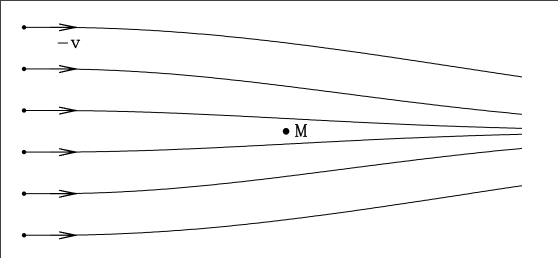
\includegraphics[width=4.5in]{dynamicalfriction.png}

\begin{equation}
	\label{}
	f_{d}\approx c\frac{G^{2}M^{2}\rho}{V_{m}^{2}}
\end{equation}
Where $c$ is a value between 20 and 200 that is comparing $v_{m}$ the relative velocities in the environment. 

For $v_{m}\gg v_{average}$ there is no dynamical friction, but collisions still provide kinetic energy.



\subsection{Measuring extragalactic distances}

\textbf{Parallax:} One can determine the distance of a star using trigonometry based on the movement of the earth around the sun. 

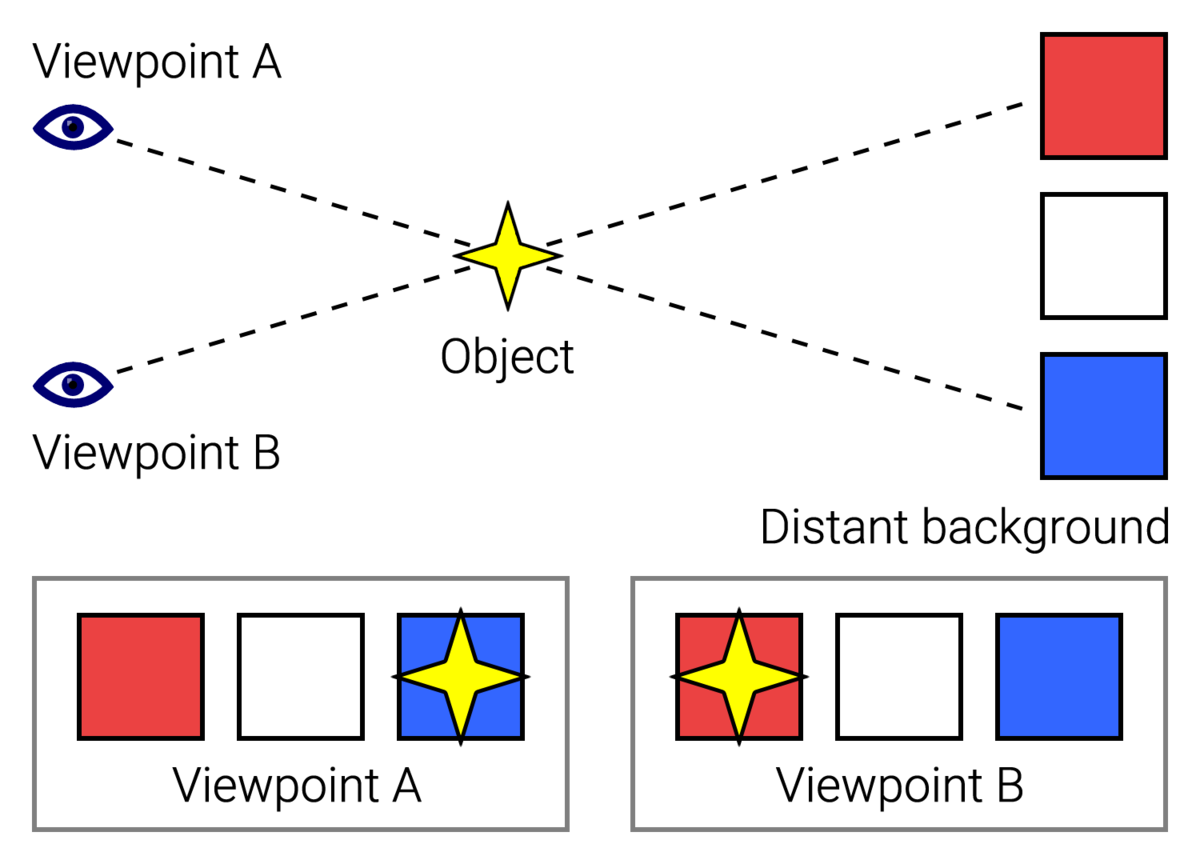
\includegraphics[width=4.5in]{parallax.png}


Using small angle approximation:
\begin{equation}
	\label{}
	p=\frac{1[Au]}{d}\quad, d=\frac{1[Au]}{p}
\end{equation}
Where p is parallax angle, i.e.\ from red to star to white box$\ldots$. For p in arcsec, d is in parsecs. For p in radians, d is in Au.

The star may have velocity in the sky due to movement of solar system, or the star itself. When plotting parallax motion this movement will be constant with the parallax motion sinusoidally modifying it. 

\hfill
\hfill


\textbf{Cepheid Variables: } stars that change radius, and therefore luminosity periodically. 

\begin{equation}
	\label{}
	M_{v}=-3.53\log(\tau_{days})-2.13+2.13(B-V)
\end{equation}
From $M_{v}$ find luminosity, then compare to apparent magnitude (obs flux) to find distance.

The (B-V) dependence indicates that there is a temperature dependence.


\hfill
\hfill

\textbf{Type Ia Supernovae: } likely white dwarves upon reaching $1.44M\odot$. Because of the similar masses of all these supernovae, their absolute magnitude is known, and can be compared to find distance. To be sure a new bright dot is a Type Ia Supernovae, one must check the spectrum, which for Ia should not have much hydrogen, and watch the magnitude over time to be sure it matches. They reach up to almost -20 magnitude, and are thus very bright and can be seen very far away. 

The supernova group and the exoplanet community are very intense and competitive.

\subsection{Expansion}
\textbf{Hubble Constant: }$H_{0}\approx71\frac{km/s}{Mpc}$. Different methods of calculating this constant


\begin{equation}
	\label{}
	z=\frac{v}{c}
\end{equation}
Peak star formation occurred at a $z\approx 2$. Including expansion of space with measured velocities indicates galaxies are moving faster than light away from each other.

Local group, gravity$\>$expansion, Virgo cluster that encompasses local group and other groups, expansion$\>$gravity


\textbf{Hot gas in intergalactic medium } has a luminosity density $[L/Volume]$, usually denoted $\mathcal{L}$


\begin{equation}
	\label{}
	\mathcal{L}=1.42 \times 10^{-40}n_{e}^{2}\cdot T^{0.5}\ [W/m^{2}]
\end{equation}


\section{Relativity}
Newtons Laws work in inertial reference frames. But, there is no way to determine the difference between an inertial and non inertial frame in the case of the freefaling box in g or the upwardly accelerating box. Relativity is concerned with \textbf{connecting} these reference frames.

\textbf{Gravitational Redshift}
\begin{equation}
	\label{}
	g=\frac{GM}{r^{2}}
\end{equation}
\begin{equation}
	\label{}
	\frac{\Delta\nu_{g}}{\nu_{0}}=\frac{-GM}{r^{2}c^{2}}
\end{equation}
Considering a photon travelling out of some gravitational potential (does this apply to other potentials?), g will change so it must be integrated.
\begin{equation}
	\label{}
	\int_{\nu_{0}}^{\nu_{\infty}}=-\int_{r_{0}}^{\infty}\frac{GM}{r^{2}c^{2}}dr
\end{equation}
pg. 620
\begin{equation}
	\label{}
	\frac{\nu_{\infty}}{\nu_{0}}=(1-\frac{2GM}{r_{0}c^{2}})^{1/2}=\frac{t_{0}}{t_{\infty}}
\end{equation}

If light emitted decreases frequency in frequency, where it is emitted from experiences a relatively slower time that where it ends up. 
Frequency decreasing is equivalent to \textbf{time slowing down.} Clocks tick slower in strong gravitational wells, \textbf{time dilation}. These phenomena are the same.

\subsection{Distances in Spacetime}

\textbf{Spacetime Interval}, $\Delta S$ is defined as the light travel distance between $t_{A}$ and $t_{B}$ minus the distance between A and B. This case is \textbf{non relativistic} and only applies to the transmission of information
\begin{equation}
	\label{}
	\Delta S^{2}=[c(t_{b}-t_{a})]^{2}-\Delta l^{2}
\end{equation}
Where $l$ is the straight line distance in Cartesian coordinates. 

If this is negative, it is outside the light cone. 

Some New terms:
\begin{enumerate}
	\item \textbf{Proper Time: $\Delta\tau$: }time between events at the same location when compared to an observed in flat spacetime, where $\frac{M}{r}=0$
	\item \textbf{Proper Distance: $\Delta\mathcal{L}=\sqrt{-(\Delta S)^{2}}$: }distance between two events that occur simultaneously ($\Delta S$) is imaginary because information cannot pass between two events with $\Delta t=0$
\end{enumerate}
dr and dt are in flat spacetime


\hfill
\hfill

Types of spacetime intervals:
\begin{enumerate}	
	\item \textbf{Lightlike (null): } $\Delta S^{2}=0$, spacetime interval of massless particle
	\item \textbf{Timelike (more time than needed): }$\Delta S^{2}>0$, any possible distance traversable of anything with mass
	\item \textbf{Spacelike: }$\Delta S^{2}<0$, cannot have causal relationship 
\end{enumerate}

\subsection{Curved Spacetime}
\begin{equation}
	\label{}
	\Delta S^{2}=(ct)^{2}-(dr)^{2}-(rd\theta)^{2}-(r\sin(\theta)d\phi)^{2}
\end{equation}
To incorporate curved spacetime we use how time changes with respect t mass. 
\begin{equation}
	\label{}
	\frac{\Delta t_{0}}{\Delta t_{\infty}}=(1-\frac{2GM}{r_{0}c^{2}})^{1/2}
\end{equation}
We can also expect that dr will change in the presence of mass
\begin{equation}
	\label{}
	dS^{2}=\bigg(cdt\sqrt{1-\frac{2GM}{rc^{2}}}\bigg)^{2}-\bigg(\frac{dr}{\sqrt{1-\frac{2GM}{rc^{2}}}}\bigg)^{2}-(rd\theta)^{2}-(r\sin(\theta)d\phi)^{2}
\end{equation}
where t and r are measured at a large distance from M.


\textbf{Proper Time}
\begin{equation}
	\label{}
	\Delta\tau=\frac{ds}{c}=dt\sqrt{1-\frac{2GM}{rc^{2}}}
\end{equation}
where
\textbf{Proper Distance} for spherical symmetry
\begin{equation}
	\label{}
	d\mathcal{L}=\sqrt{-(dS^{2})}=\frac{dr}{\sqrt{1-\frac{2GM}{rc^{2}}}}
\end{equation}
Spatial difference is larger than dr ($d\mathcal{L}>dr$), because it is curved.


\subsection{Gravitational Lensing}
\begin{equation}
	\label{}
	\phi=\frac{4GM}{r_{0}c^{2}}
\end{equation}

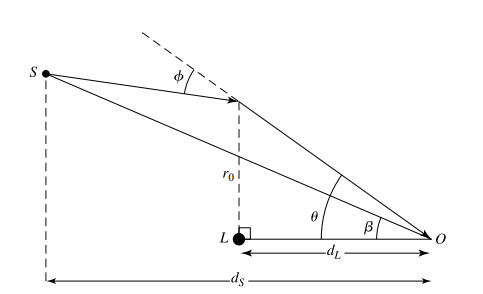
\includegraphics[width=4.5in]{gravlensing.png}


Only works for `double image' gravitational lensing


\section{Cosmology}

Hubble Parameter
\begin{equation}
	\label{}
	H=\frac{1}{R}\frac{dR}{dt}
\end{equation}

\subsection{Newtonian Cosmology}


Critical density is given by
\begin{equation}
	\label{}
	\rho_{c}=\frac{3H_{0}^{2}}{8\pi G}
\end{equation}
The term $\Omega$ describes a universe's density relative to the critical density. 
\begin{equation}
	\label{}
	\Omega=\frac{\rho}{\rho_{c}}
\end{equation}
\begin{enumerate}
	\item $\Omega=1$ steady state, balanced	
	\item $\Omega<1, E>0$, unbounded, expansion forever
	\item $\Omega>1, E<0$, bounded, collapse
\end{enumerate}

\textbf{Defining 2 new terms useful for General Relativity and non-zero newtonian models}
\begin{enumerate}
	\item k: units of $\mbox{length}^{-2}$
	\item $\varpi$: $r(t_{0})$, `varpi' radius of current shell, always our time because $Z$ is relative to time now. See definition of $R(t)$ 
\end{enumerate}

\begin{equation}
	\label{}
	-kc^{2}\varpi^{2}=v^{2}-\frac{8}{3}\pi G\rho r^{2}
\end{equation}

If $E=0$, then $k=0$

The cosmological constant says that two shells will take the same amount of time to double in radius.
Let
\begin{equation}
	\label{}
	r(t)=\varpi R(t)
\end{equation}
where $R(t)$ is a dimensionless scale factor defined by the redshift of the universe
\begin{equation}
	\label{}
	R=\frac{1}{1+Z}
\end{equation}
Including pressure in this function and the first law of thermal dynamics this equation can be derived
\begin{equation}
	\label{}
	\frac{d^{2}R}{dt^{2}}=-\frac{4}{3}\pi G(\rho + \frac{3P}{c^{2}})R
\end{equation}
Is the acceleration equation. Unfortunately, the actual pressure of the universe is too great for this and it does not actually work.


Friedmann Equation:
\begin{equation}
	\label{}
	\bigg[\big(\frac{1}{R}\frac{dR}{dt}\big)^{2}-\frac{8}{3}\pi G(\rho_{m}+\rho_{r})\bigg]R^{2}=-kc^{2}
\end{equation}



\subsection{Pressure expansion model, 2 component universe}

What is the relationship between density and pressure, what is the density made of?

\textbf{Baryonic Matter} (all luminous matter): ideal gas law!
\begin{equation}
	\label{}
	P=\frac{Nk_{b}T}{\bar{m}}\rho,
\end{equation}
For neutral H in current-sized universe, $P\approx 2.5 \times 10^{-13}\approx 0$

\textbf{Radiation: } A bunch of ultrarelativistic particles. Energy density of thermal emission:
\begin{equation}
	\label{}
	u_{rad}=aT^{4},\quad \rho=\frac{u_{rad}}{c^{2}},\quad
\end{equation}
\begin{equation}
	\label{}
	 P_{rad}=\frac{1}{3}\rho_{rad}c^{2}
\end{equation}
Radiation Equation of State.


Where a is the radiation constant, $u_{rad}$ is the energy density


finding how $\rho_{rad}$ changes with $R$ can allow a more complete model. $P_{rad}$ can be substituted in the fluid equation:
\begin{equation}
	\label{}
	\frac{d(\rho)R^{2}}{dt}=-\frac{P}{c^{2}}\frac{d(R^{2})}{dt}
\end{equation}
giving (after some algebra and integration)
\begin{equation}
	\label{}
	\rho_{rad}(R)=\frac{\rho_{0,\mbox{rad}}}{R^{4}}	
\end{equation}
Where $\rho_{0,\mbox{rad}}$ is radiation density right now.
Compare to matter density: $\rho_{m}=\frac{\rho_{m,0}}{R^{3}}$. At some point $R\approx 10^{-4}$, matter density surpassed radiation density

\begin{equation}
	\label{}
	\Omega_{m,0}=\frac{\rho_{m}}{\rho_{c,0}},\quad \Omega_{r,0}=\frac{\rho_{rad}}{\rho_{c,0}}
\end{equation}

Shortly after this happened, \textbf{recombination happened, }and the universe became transparent


\subsection{Relativistic Cosmology}
\textbf{Friedmann-Robertson-Walker Metric}
\begin{equation}
	\label{}
	ds^{2}=(cdt)^{2}-R^{2}(t)\bigg[	\big(\frac{d\varpi}{\sqrt{1-k\varpi^{2}}}\big)^{2}+(\varpi d\theta)^{2}+(\varpi\sin(\theta)d\theta)^{2}	\bigg]
\end{equation}
\begin{enumerate}
	\item $t$ is cosmic time, time at infinity
	\item $R(t)$ is scale factor
	\item $k$ is the curvature constant
	\item $\varpi,\theta,\phi$ are comoving coordinates
\end{enumerate}

\textbf{Friedmann Equation with Cosmological Constant}
\begin{equation}
	\label{}
	\bigg[\big(\frac{1}{R}\frac{dR}{dt}\big)^{2}-\frac{8}{3}\pi G(\rho_{m}+\rho_{r})-\frac{1}{3}\Lambda c^{2}\bigg]R^{2}=-kc^{2}
\end{equation}
For a positive $\Lambda$, an outward force is supplied to balance gravitational collapse. This is how Einstein formulated it.

In a Newtonian Model:
\begin{equation}
	\label{}
	u_{\Lambda}=-\frac{1}{6}\Lambda m c^{2}r^{2}
\end{equation}
Represents the energy density of dark energy


Acceleration equation
\begin{equation}
	\label{}
	\frac{d^{2}R}{dt^{2}}=\bigg(-\frac{4}{3}\pi G \big[\rho_{m}+\rho_{r}+\frac{3(P_{m}+P_{r})}{c^{2}}\big]+\frac{1}{3}\Lambda c^{2}\bigg)
\end{equation}

Density of dark energy
\begin{equation}
	\label{}
	\rho_{\Lambda}=\frac{\Lambda c^{2}}{8\pi G},\quad P_{\Lambda}=-\rho_{\Lambda}c^{2}
\end{equation}
Dark energy is then added to the equations we were working with previously. This can be found on pages 1192-1193.

\begin{equation}
	\label{}
q(t)=\frac{1}{2}\Omega_{m}(t)+\Omega_{r}(t)-\Omega_{\Lambda}(t)
\end{equation}


\pagebreak
\section{Useful Notes}
\begin{enumerate}
	\item When doing a triple spherical integral for a spherical symmetric body, $\int f(x) \cdot 4\pi r^{2}dr$ can be used rather than the triple integral.	
\end{enumerate}

\end{document}

